\documentclass{article}
\usepackage[utf8]{inputenc}
\usepackage[margin=1.0in]{geometry}
\usepackage{amsmath}
\usepackage{amssymb}
\usepackage{fancyhdr}
\usepackage{physics}
\usepackage{wrapfig}
\usepackage{hyperref}
\usepackage{multirow}
\usepackage{amsthm}
\usepackage{pgfplots}
\usepackage{float}

\pgfplotsset{compat=1.16}



\renewcommand{\thesubsection}{\thesection\Alph{subsection}}
\renewcommand\qedsymbol{\square}



\title{Particle Physics PS3}
\author{Joe Crowley}
\date{October 2020}

\pagestyle{fancy}
\renewcommand{\headrulewidth}{0pt}
\renewcommand{\footrulewidth}{1pt}

\fancyhf{}
\rhead{
Joe Crowley \\
Physics 225 \\
Problem Set 3\\
}
\rfoot{Page \thepage}

\begin{document}  



\section{The famous $q^{2}$ variable.}
\textit{The quantity $q^{2}=\left(p_{i}-p_{f}\right)^{2},$ where $p_{i}$ and $p_{f}$ are the 4-momenta of a particle before and after scattering from some target particle or system, plays a major role in many processes in particle physics. Consider a low-mass beam particle, such as an electron, whose mass is negligible compared to its energy. Let the initial 3 -momentum direction of the electron be aligned along the $x$ -axis and the final 3 -momentum direction be at an angle $\theta$ with respect to the $x$ -axis, in the $x y$ plane.}

\subsection{}
\textit{Write down the components of $p_{i}$ and $p_{f}$ in terms of the electron's energy and direction only. In other words, given that $m_{e}$ is negligible, you can use $|\vec{p}|=E$}

\begin{align*}
    p_i &= (E_i, E_i,0,0)\\
    p_f &= (E_f, E_f \cos{\theta},E_f \sin{\theta},0)\\
\end{align*}




\subsection{}
\textit{Compute $q^{2}$ and make a sketch of $q^{2}$ as a function of $\cos \theta$.}
\begin{align*}
    q^{2}&=\left(p_{i}-p_{f}\right)^{2}\\
    &=p_{i}^{2}+p_{f}^{2}-2 p_i p_{f}\\
    &=p_{i}^{2}+p_{f}^{2}-2\left(E_{i} E_{f}-\vec{p_i} \cdot \vec{p}_{f}\right)\\
    &=p_{i}^{2}+p_{f}^{2}-2 E_{i} E_{f}+2\abs{\vec{p}_{i}} \abs{\vec{p}_{f}}  \cos \theta\\
    &=p_{i}^{2}+p_{f}^{2}-2 E_{i} E_{f}(1-\cos \theta)
\end{align*}
\begin{figure}[H]
    \centering
    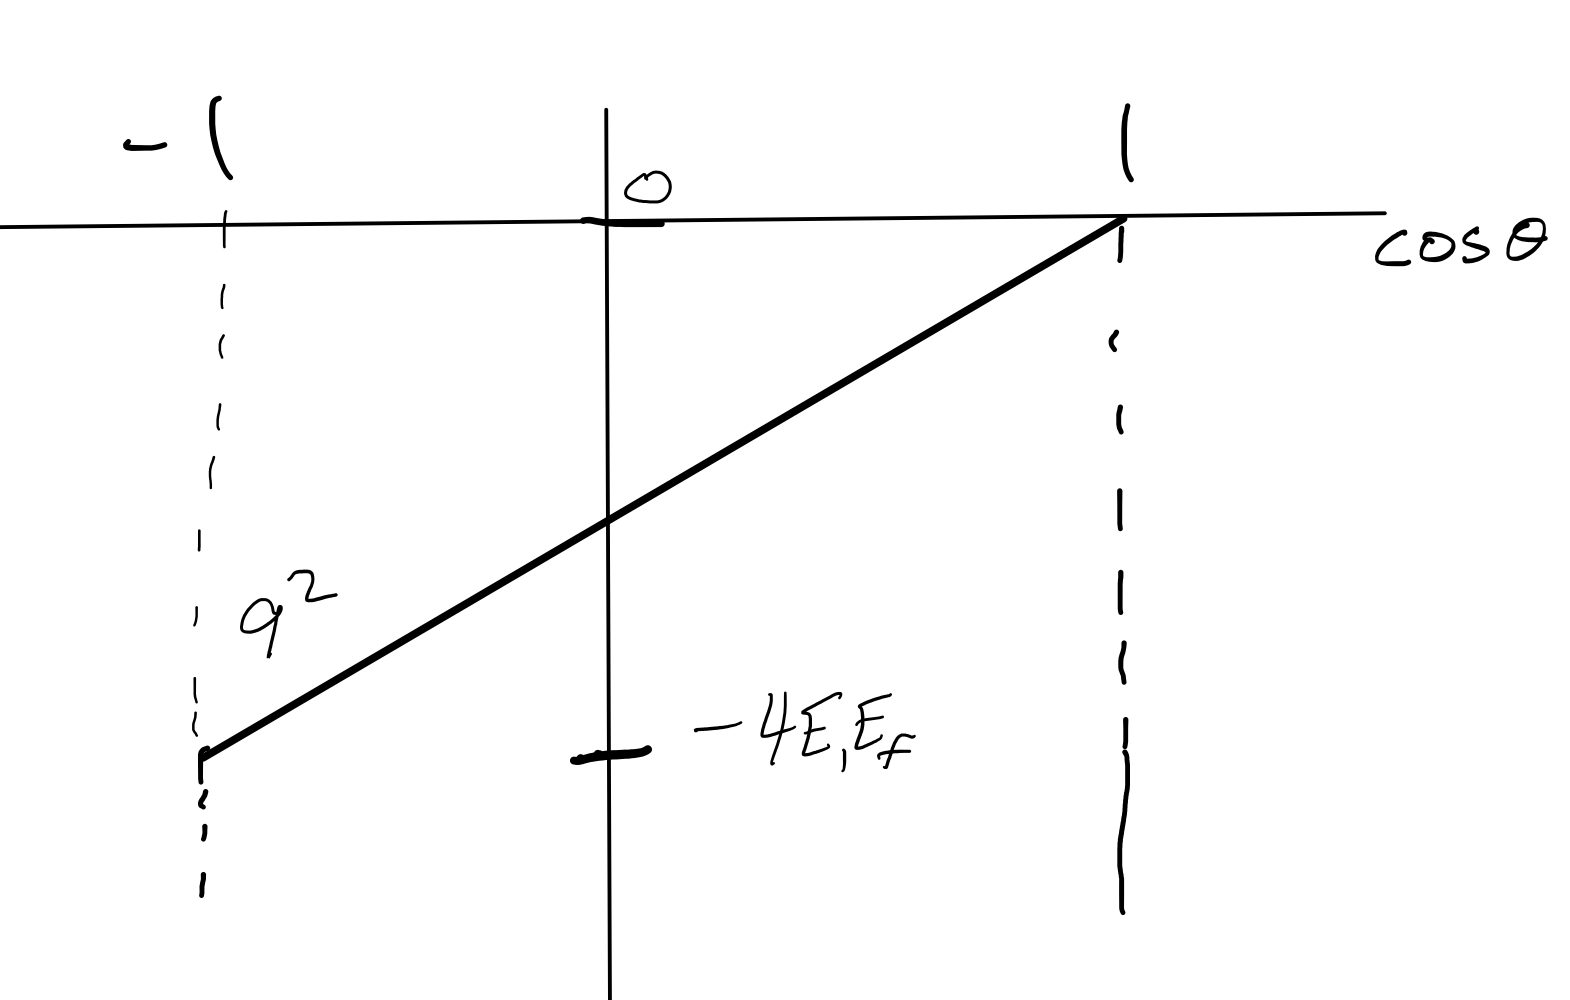
\includegraphics[width=0.4\textwidth]{figures/problem1.png}
    \label{fig:my_label}
\end{figure}

\subsection{}
\textit{Use a trigonometric half-angle formula to express $q^{2}$ in terms of $\sin \theta / 2$ Look up the Rutherford scattering formula and comment on its angular dependence. This is not a coincidence, as we will see when we study Feynman diagrams.}

\begin{align*}
    q^{2}&=p_{i}^{2}+p_{f}^{2}-2 E_{i} E_{f}\left(2 \sin ^{2} \frac{\theta}{2}\right)\\
    &\approx -4 E_{i} E_{f} \sin ^{2} \frac{\theta}{2}
\end{align*}

The rutherford scattering differential cross section has $1/\sin^4{\theta}$ dependence, is $\frac{d \sigma}{d \Omega} \propto \frac{1}{q^{4}}$?


\newpage


\section{}
\textit{Give short answers to the following simple questions. For True/False questions, please justify your answer with a short explanation.}



\subsection{}
\textit{ A muon has a mean lifetime of $2.2 \mu \mathrm{s}$ in its rest frame. Assuming that a beam of muons is produced with $p=5 \mathrm{GeV},$ what is the mean distance that the muons travel in the lab before decaying?}
\begin{align*}
    \Delta x & =\beta \gamma \tau\\
    &=\frac{p}{m_{\mu}} \tau\\
    &=\frac{5 \mathrm{G e V}}{0.1 \mathrm{G e V}} 2.2 \times 10^{-6} \text {seconds }\\
    &\approx 33 \mathrm{km}
\end{align*}

\subsection{}
\textit{True or False: if two photons are traveling in the same direction, then the invariant mass associated with the two-photon system is zero, regardless of the energies of the photons.}

\textbf{True}. A photon (or collection of photons moving in the same direction) have no CM frame, because the lorentz invariant $p^2 = E_\gamma ^2$ would be 0 in the CM frame. 

\subsection{}
\textit{True or False: if a beam of electrons with energy $E_{e}$ is incident on a target particle with mass $m_{T}$ in the lab frame, then, for $E_{e}>>m_{t}, m_{e},$ the total energy in the CM frame rises linearly with the electron beam energy.}
\begin{align*}
    \left(\left(E_{e}, E_{e}, 0,0\right)+\left(m_{t}, 0,0,0\right)\right)^{2}&=E_{C M}^{2}\\
    \left(E_{e}+m_{t}\right)^{2}-E_{e}^{2}&=E_{CM}^{2}\\
\end{align*}

\begin{align*}
    m_{t}^{2}+2 E_e m_{t}&=E_{CM}^{2}\\
    E_{CM} &\approx \sqrt{2 m_{t} E_{e}}\\
\end{align*}
\textbf{False.} $E_{CM} \propto \sqrt{E_e}$

\subsection{}
\textit{ True or False: The set of positive integers $i=1,2,3, \ldots$ forms a group under the operation of ordinary multiplication. (Be sure to consider all four group properties.)}

\textbf{False.} The set of positive integers does not form a group undar ordinary multiplication because there exist no inverse elements, however it does satisfy the axioms of closure associativity, and identity.

\subsection{}
\textit{ True or False: The set of all $2 \times 2$ unitary matrices $U$ with det $U=1$ forms a group under the operation of matrix multiplication.}

Closure: 
\begin{align*}
    \exists(U_k) \, \forall(U_i,U_j): U_i U_j &= U_k\\
    \mathrm{det}(U_i U_j) &= \mathrm{det}(U_i)\mathrm{det}( U_j)\\
    &= 1\\
    &\\
    U_{i} U_{j}&=U_{k}\\
    (U_{i} U_{j})^\dagger &=U_{k}^\dagger\\
    U_{j}^\dagger U_{i}^\dagger &=U_{k}^\dagger\\
    U_{j}^{-1} U_{i}^{-1} &=U_{k}^\dagger\\
    &\\
    U_{k}^{\dagger} U_{k} &=U_{j}^{-1} U_{i}^{-1} U_{i}U_{j}\\
    &=1\\
    &\\
    U_{k}^{\dagger} &=  U_{k}^{-1}
\end{align*}


Associativity: Trivially holds for $n\times n$ matrices.

Identity: $2\times 2$ diagonal matrix of $1's$.

Inverse: $\forall U_i \, \exists U_i^{-1} = U_i^\dagger:  U_i^{-1}  U_i = U_i^{\dagger} U_i = 1$

\newpage


\section{Thinking about hadrons.}
\subsection{}
\textit{The $J / \psi(1 S)$ is a bound state of $c$ and $\bar{c}$ quarks. When the $J / \psi$ decays, these quarks must annihilate, rather than forming two charm mesons, e.g., $D^{0}$ and $\bar{D}^{0} .$ Explain why this is. (Hint: at this point in the course, the answer has to be very simple.) }

The mass of the $J / \psi(1 S)$ is less than the mass of $D^{0}$ and $\bar{D}^{0}$. This forces $J / \psi(1 S)$ to decay via $c\bar c$ annihilation.  


\subsection{}
\textit{The $\psi(3770)$ is able to decay into two charm mesons. What is the value of the orbital angular momentum $L$ in the $D^{0} \bar{D}^{0}$ or $D^{+} D^{-}$ system? Explain. }    

$\psi(3770)$ has $ J^{P}=1^-$, $ D^{0}$ has $ J^{p}=0^-$. Conservation of angular momentum implies for $D^{0} \bar{D}$ that $L=1$.


\subsection{}
\textit{The $D^{0}$ meson can undergo the decay $D^{0} \rightarrow K^{+} \pi^{-}$. What is the valuie of the orbital angular momentum $L$ in the $K^{+} \pi^{-}$ system? Explain.}

$D^{0}$ has $J^{P}=0^{-}$, $K^{+}$ has $J^{P}=0^{-}$, $\pi^{+}$ has $J^{p}=0^{-}$. L must be 0 for $K^{+} \pi^{+}$ system.


\subsection{}
\textit{Consider a baryon, which is made of quarks $q_{1} q_{2} q_{3}$. For the spin ( $S$ ) part of the baryon state vector (not orbital angular momentum part), what are the possible direct-product states of a three-quark system? How many such states are there? Now find the states with definite total $S$ and express them in terms of the direct product states using Clebsch-Gordon coefficients from the Particle Data Book. How many such states are there?}

$$ \ket{j, m_j} = \ket{s_1, m_1}\otimes \ket{s_2, m_2}\otimes \ket{s_3, m_3}$$

For values $s_i = \frac{1}{2}, m_i = \pm \frac{1}{2}$, the allowed values of $j$ are $\frac{1}{2},\frac{3}{2}$, which have values of $m_j = \{\pm \frac{1}{2}\},\{\pm \frac{1}{2}, \pm \frac{3}{2}\}$, for a total of 8 states. These states are found by starting in the $\ket{j, m_j} = \ket{\frac{3}{2}, \frac{3}{2}}$ state and applying the $J^- = S_1^-+S_2^-+S_3^-$ operator. Because of the many ways to permute the three direct product states, the $\ket{\frac{1}{2}, \pm \frac{1}{2}}$ states are written with two antisymmetric permutations. the $\ket{\frac{3}{2}, \pm \frac{3}{2}}$ state is symmetric under permutations of any two quarks. 

\newpage

\section{Neutral pion decay into two photons: $\pi^{0} \rightarrow \gamma \gamma$}
\textit{A $\pi^{0}$ meson with energy $E_{\pi}=0.75 \mathrm{GeV}$ in the lab frame decays in flight into two photons. The $\pi^{0}$ flight direction is along the $x$ axis. For simplicity, you make assume that the photon momentum vectors lie in the $x y$ plane. (This does not change the answers for the questions below.)}


\subsection{}
\textit{What is the branching fraction for the decay $\pi^{0} \rightarrow \gamma \gamma ?$}

$$\frac{\Gamma_i}{\Gamma} = (98.823 \pm 0.034) \%$$


\subsection{}
\textit{Compute the velocity $\beta=v / c$ of the pion in the lab frame.}
\begin{align*}
    \frac{1}{\sqrt{1-\beta ^2}}&= \frac{E_\pi}{m_\pi}\\
    \beta &= \frac{\sqrt{E_\pi^2-m_\pi^2}}{E_\pi}\\
    &= \frac{\sqrt{(0.75 \mathrm{GeV})^2-(0.1349770\mathrm{GeV})^2}}{0.75 \mathrm{GeV}}\\
    &= 0.983672
\end{align*}

$$\boxed{\beta = 0.983672}$$

\subsection{}
\textit{In the $\pi^{0}$ rest frame, the angle of one of the two photons $\left(\gamma_{1}\right)$ with respect to the $x^{\prime}$ axis is $\theta_{1}^{\prime}=45^{\circ} .$ Compute the angle $\theta_{1}$ of $\gamma_{1}$ with respect to the $x$ axis in the lab frame.}


\begin{align*}
    E^{\mathrm{Lab}}&=\gamma E^{\mathrm{rest}}+\beta \gamma p_{x}^{\mathrm{rest}}\\
    &\\
    E^{\mathrm{rest}}&=\frac{1}{2} E_{\pi}^{\mathrm{rest}}=\frac{1}{2} m_{\pi}\\
    p_{x}^{\mathrm{rest}}&=\left|p^{\mathrm{rest}}\right| \cos \theta^{\mathrm{rest}}\\
    E^{\mathrm{Lab}}&=\gamma E^{\mathrm{rest}}+\beta \gamma \frac{1}{2} m_{\pi} \cos \theta^{\mathrm{rest}}\\
\end{align*}

$$E^{\mathrm{lab}}=\frac{1}{2} m_{\pi} \gamma\left(1+\beta \cos \theta^{\mathrm{rest}}\right)$$

\begin{align*}
    \tan \theta^\mathrm{Lab}&=\frac{p_{y}^\mathrm{Lab}}{p_{x}^\mathrm{Lab}}\\
    &=\frac{ \sin \theta^{\mathrm{rest}}}{\gamma\beta  \cos \theta^{\mathrm{rest}}}\\
    &= \frac{\sqrt{1-\beta^{2}}}{\beta} \frac{\sin \theta^{\mathrm{rest}}}{  \cos \theta^{\mathrm{rest}}}
\end{align*}

$$\boxed{\theta^\mathrm{Lab} = \arctan{\left(\frac{\sqrt{1-\beta^{2}}}{\beta} \frac{\sin \theta^{\mathrm{rest}}}{  \cos \theta^{\mathrm{rest}}}\right)} = \frac{\sqrt{1-0.983672^2} \sin (45 {}^{\circ})}{0.983672 \cos (45 {}^{\circ})}= 0.182958}$$

\subsection{}
\textit{Is this angle larger or smaller than $\theta_{1}^{\prime} ?$ Explain why this should be the case.}

This is a much smaller angle than $\theta^{\mathrm{rest}}$, which is expected because the photons should have a uniform angular distribution in the rest frame, and the boost will shift small angles toward the x-axis, shown in the plot below. 

\begin{figure}[H]
    \centering
    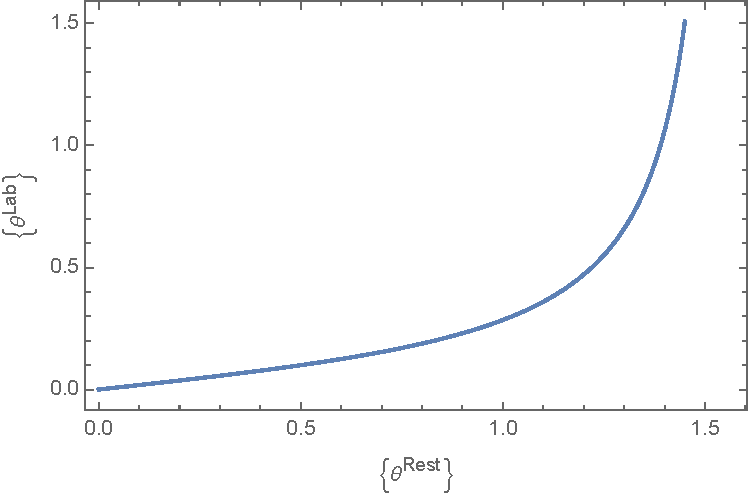
\includegraphics[width=0.6\textwidth]{figures/thetaRestThetaLab.pdf}
    \caption{Plot of $\theta^{\mathrm{rest}}$ vs. $\theta^{\mathrm{Lab}}$ for $\beta = 0.983672$.}
    \label{fig:my_label}
\end{figure}

\subsection{}
\textit{Now, consider a beam of a large number of $\pi^{0}$'s all with the same energy as in the preceding parts. In the $\pi^{0}$ rest frame, the photons are emitted isotropically. What is the distribution of the photon energies in the lab frame? Be sure to discuss both the shape and the endpoint values of this distribution.}

The angular distribution in the CM frame will be uniform in $\cos \theta^{\mathrm{rest}}$, with endpoint values $\frac{1}{2} m_{\pi} \gamma(1\pm \beta)$

\begin{figure}[H]
    \centering
    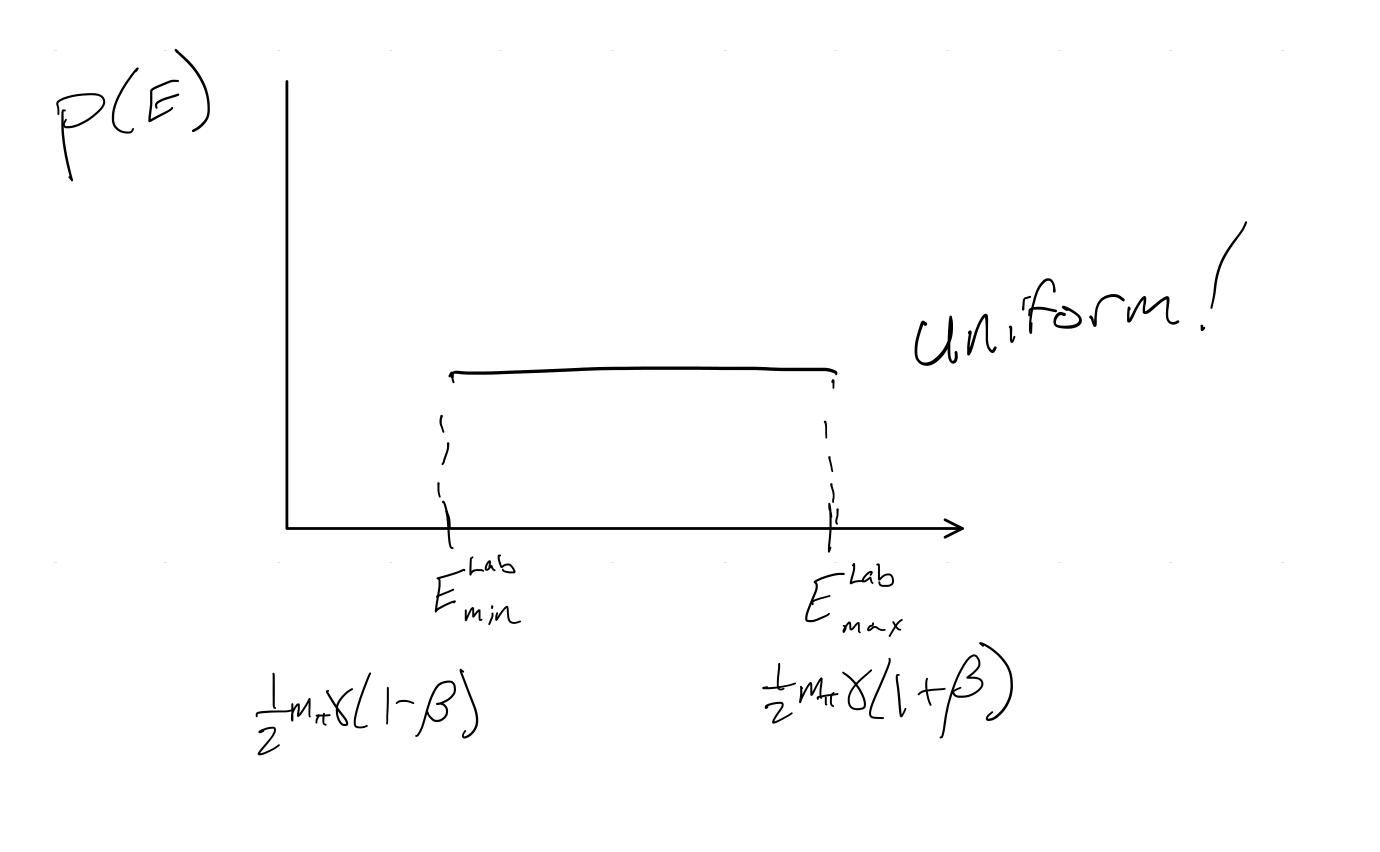
\includegraphics[width=0.6\textwidth]{figures/angularPiDistribution.png}
    \label{fig:my_label}
\end{figure}

\newpage

\section{Decay-time distributions and the Breit-Wigner.}
\subsection{}
\textit{The mean lifetime of a particle is $\tau$. Calculate the probability for the particle to decay between time $t=0$ and time $t=5 \tau$}


If the survival probability is given by $e^{-\frac{t}{\tau}}$, the decay probability is $1-e^{-\frac{t}{\tau}} = 1-e^{-5}= 0.993262$


$$\boxed{P(\mathrm{decay \, in } \,5\tau\, \mathrm{seconds}) =0.993262 }$$

\subsection{}
\textit{The mean lifetime of the proton is known to be greater than about $10^{33}$ years. Assuming that this value is in fact the mean lifetime of the proton, calculate the probability for one proton to decay during a 5 year period over which an experiment operates. You may use an appropriate approximation.}

Using the approximation $e^x \approx 1 + x$,

$$\boxed{P(\mathrm{decay \, in } \,5\, \mathrm{years}) =1-e^{-\frac{1}{2\times 10^{32}}}\approx 5 \times 10^{-33} }$$

\subsection{}
\textit{The proton mass is $m_{P} \approx 1.67 \times 10^{-27} \mathrm{kg} .$ Based on your answer to the previous part, estimate the mass of a detector that you should build to expect 10 protons to decay over this operational period. You may assume that the detector is made of half protons and half neutrons and that any proton that decays would be detectable.}

Based on my previous calculation, I would need approximately $10^{34}$ protons to expect to observe 10 decays. Assuming the mass of water is $50\%$ protons, $50\%$ neutrons, the detector should be about 
$$\boxed{10^{34} (m_p + m_n) = 3.347549397\times 10^7\text{kg}}$$


\subsection{}
\textit{A quantum system has states $i=0,1,2,3,$ where $i=0$ is the ground state and is stable. Transitions occur within this system the rates $\Gamma_{f i},$ where $i$ is the initial state and $f$ is the final state involved in the transition:
$$
\begin{aligned}
\Gamma_{23}=0.5, \quad \Gamma_{13}=7.5, \;& \Gamma_{03}=2.7 \\
\Gamma_{12}=2.5, \; & \Gamma_{02}=4.3 \\
&\Gamma_{01}= 8.0
\end{aligned}
$$
where all of the partial decay widths are given in MeV. In terms of these quantities, calculate the mean lifetime for each state and list the states in order of increasing lifetime.}
$$ \tau_i = \frac{1}{\Gamma_{i}}$$

\begin{align*}
    \tau_{23} &= \frac{1}{\Gamma_{23}} = 2 \\
    \tau_{13} &= \frac{1}{\Gamma_{13}} =0.133333 \\
    \tau_{03} &= \frac{1}{\Gamma_{03}} = 0.37037\\
    \tau_{12} &= \frac{1}{\Gamma_{12}} = 0.4 \\
    \tau_{02} &= \frac{1}{\Gamma_{02}} = 0.232558\\
    \tau_{01} &= \frac{1}{\Gamma_{01}} = 0.125
\end{align*}



\subsection{}
\textit{Suppose that two different types of particles $X$ and $Y$ have mean lifetimes $\tau_{X}$ and $\tau_{Y},$ and that, for some physics reason, we know that $\Gamma(X \rightarrow$ $\left.f_{X}\right)=\Gamma\left(Y \rightarrow f_{Y}\right),$ where $f_{X}$ and $f_{Y}$ are possible decay final states for the respective decays of particles $X$ and $Y .$ True or False:
$$
\frac{B\left(X \rightarrow f_{X}\right)}{B\left(Y \rightarrow f_{Y}\right)}=\frac{\tau_{X}}{\tau_{Y}}
$$
Explain your answer with a short calculation.}

True.
$$ B_i = \frac{\Gamma_i}{\Gamma_{tot}} $$

\begin{align*}
    B^X &= \frac{\Gamma}{\Gamma_{tot}^X} = \tau_X \Gamma \\
    B^Y &= \frac{\Gamma}{\Gamma_{tot}^Y} = \tau_Y \Gamma \\
    \frac{B^X}{B^Y}& = \frac{\tau_X}{\tau_Y}
\end{align*}

\subsection{}
\textit{True or False: the observed width of a $Z$ boson, reconstructed in a decay channel $Z \rightarrow f f,$ where $f$ is a particular type of fermion, reflects the decay rate for that particular decay mode. That is, if you look at the distribution of $Z$ -boson masses in a sample of decays in which $Z \rightarrow c \bar{c},$ the full-widthat-half-maximum of the Breit-Wigner line shape will in fact be $\Gamma(Z \rightarrow c \bar{c})$ not the total decay width of the $Z .$ Explain your answer.}

False. For every decay mode, the full width at half maximum corresponds to the mean lifetime of the sample, but the sample can decay in many different ways. In any decay mode, the experimentally observed width of the distribution wil be $\frac{1}{\tau}$ and the branching fraction for the particular mode will be 

$$ B_i = \frac{N_\mathrm{observed\, decays\, in\, mode\, i}}{N_\mathrm{observed\, decays\, total}}$$

\newpage

\section{Gravity with compactified dimensions.}
\textit{In an interesting speculation, it has been suggested (Arkani-Hamad $1998,1999,$ Antoniadis $e t\, al.$ 1998 ) that the weakness of gravity as observed our (apparently) three-dimensional world could be due to the fact that gravity actually extends into additional 'compactified' dimensions (that is, dimensiong which have the geometry of a circle, rather than of an infinite line). For the particles and forces of the Standard Model, however, such leakage into extra dimensions has to be confined to currently probed distances, which are of order $M_{\mathrm{W}}^{-1}.$}

\subsection{}
\textit{Consider Newtonian gravity in $(3+d)$ spatial dimensions. Explain why you would expect that the gravitational potential will have the form of (1.36), 
$$
V_{\mathrm{N}, 3+d}(r)=-\frac{m_{1} m_{2} G_{\mathrm{N}, 3+d}}{r^{d+1}}
$$
[Think about how the ``1/r" fall-off of the force is related to the surface area of a sphere in the case $d=0 .$ Note that the formula works for $d=-2 !$ What happens in the case $d=-1 ?]$}


Analogously with electromagnetism, a surface integral should give the flux of the field lines, a scalar. in 2 dimensions, that's 

\begin{align*}
    \oint_{\mathrm{S^2}}\left(\frac{e}{R^{2}} \hat{r}\right) \cdot \hat{r} d s &=\oint \frac{e}{R^{2}} R^{2} d \Omega\\
    &= 4 \pi e,
\end{align*}
which implies that in two dimensions $d = -1$. It is reasonable that a volume element in $3+d$ dimensions would be bounded by a $3 + d - 1$ dimensional surface. The force then could go as $\frac{1}{r^{2+d}}$ and the potential would go as $F \cdot r \propto \frac{1}{r^{1+d}}$

\subsection{}
\textit{Show that $G_{\mathrm{N}, 3+d}$ has dimensions (mass) $^{-(2+d)} .$ This allows us to introduce the 'true' Planck scale - i.e. the one for the underlying theory in $3+d$ spatial dimensions $-$ as $G_{\mathrm{N}, 3+d}=\left(M_{\mathrm{P}, 3+d}\right)^{-(2+d)}$}

\begin{align*}
    \left[G_{N, 3 + d}\right]&=\left[V_{N, 3+d}(r)\right]\left[r^{1+d}\right]\left[M^{-2}\right]\\
    &=M M^{-(1+d)} M^{-2}
\end{align*}

$$\boxed{\left[G_{N, 3 + d}\right] = M^{-(2 + d)}}$$

\subsection{}
\textit{Now suppose that the form (1.36) only holds when the distance $r$ between the masses is much smaller $R,$ the size of the compactified dimensions. If the masses are placed at distances $r \gg R,$ their gravitational flux cannot continue to penetrate into the extra di- mensions, and the potential (1.36) should reduce to the familiar three-dimensional one; so we must have
$$
V_{\mathrm{N}, 3+d}(r \gg R)=-\frac{m_{1} m_{2} G_{\mathrm{N}, 3+d}}{R^{d}} \frac{1}{r}
$$
Show that this implies that
$$
M_{\mathrm{P}}^{2}=M_{\mathrm{P}, 3+d}^{2}\left(R M_{\mathrm{P}, 3+d}\right)^{d}
$$}

This form of $V_{\mathrm{N}, 3+d}(r \gg R)$ implies that $\frac{G_{N, 3+d}}{R}=G_{N}$.
\subsection{}
\textit{Suppose that $d=2$ and $R \sim 1 \mathrm{mm}$ : what would $M_{\mathrm{P}, 3+d}$ be, in TeV? Suggest ways in which this theory might be tested experimentally. Taking $M \mathrm{p}, 3+d \sim 1 \mathrm{TeV},$ explore other possibilities for $d$ and $R$.}
$M \mathrm{p}, 3+d \sim 1 \mathrm{TeV},$
\newpage


\section{Monte Carlo simulation. (Does not need to be done with ROOT.)}
\textit{ Here you develop some techniques that you will use in future problems sets to study various probability distributions. Find a random number generator that will give you (each time you call it) a random number uniformly distributed between 0 and $1 .$ You can use these random numbers to generate any other continuous probability distribution using the following method:}



\subsection{}
\textit{Pick a probability (density) distribution that you wish to simulate. (A simple example would be a gaussian.) We call your chosen probability density function $p(x) .$ This is also called the parent distribution. Your goal is to generate a sample drawn from this parent distribution. This will help you appreciate the crucial distinction between the parent distribution (the limiting case of what you would get with infinite sample size) and a sample, which could represent an experimental measurement. One point to realize is that the mean that you measure from the sample is not in general the same as the true mean of the parent distribution; instead it is an estimator of the true mean, and it has an associated uncertainty.}


\subsection{}
\textit{Next, find the value of $x=x_{\text {mode }}$ that gives the maximum value $p_{\max }$ of $p(x)$ for all $x .$ This value of $x$ is called the mode of the distribution.}


\subsection{}
\textit{Next, generate a set of $n$ random numbers between 0 and $1 .$ Call these $r_{1}$ $r_{2}, \ldots r_{n} .$ You should try two experiments, one with $n=20$ and one with $n=100$ or greater.}



\subsection{}
\textit{Find the minimum value of $x\left(x_{\min }=a\right)$ and the maximum value of $x$ $\left(x_{\max }=b\right)$ such that outside the interval $[a, b]$ the function $p(x)$ is smaller than you care about. You might chose $[a, b]$ to get $99.9 \%$ of the total integrated probability in $p(x) .$ Then, map each of your random numbers $r_{i}$ onto the interval $[a, b]$ with the transformation $x_{i}=a+(b-a) r_{i} .$ For $r_{i}=0$ this gives $x_{i}=a$ and for $r_{i}=1$ this gives $x_{i}=b$}



\subsection{}
\textit{For each $x_{i},$ compute $\beta_{i}=p\left(x_{i}\right) / p\left(x_{\text {mode }}\right)$.}


\subsection{}
\textit{For each value of $i,$ generate a second random number $s_{i}$ uniformly between 0 and $1 .$ If $\beta_{i} \geq s_{i}$ KEEP the corresponding value of $x_{i} ;$ otherwise reject it. (This is called the "rejection method" for generating a distribution.)}



\subsection{}
\textit{Make a histogram of all the retained values of $x_{i} .$ As you increase the number of random numbers $r_{i}$ generated, your histogram will get closer and closer to the parent probability distribution. However, it's useful to do the exercise for small sample sizes when you are simulating an experiment with a modest data sample.}


\subsection{}
\textit{Explain why this method works.}

\end{document}
